\documentclass[11pt]{article}

\usepackage{scrextend}
\usepackage[a4paper, margin = 1.25in,footskip =0.25in]{geometry}
\usepackage{enumitem}
\usepackage{alltt}
\usepackage{amsmath}
\usepackage{amssymb}
\usepackage{amsthm}
\usepackage{mathtools}
\usepackage{amsmath}
\usepackage{graphicx}

\newcommand{\C}{\mathbb{C}}
\newcommand{\Q}{\mathbb{Q}}
\newcommand{\R}{\mathbb{R}}
\newcommand{\Z}{\mathbb{Z}}

\graphicspath{ {images/} }

\DeclarePairedDelimiter\ceil{\lceil}{\rceil}
\DeclarePairedDelimiter\floor{\lfloor}{\rfloor}

\usepackage{times}

\begin{document}
\begin{flushleft}
	Rowan Lochrin \\
	CSC445 - Alon Efrat\\
	4/2/18 \\
	Homework 4
\end{flushleft}
\begin{enumerate}
		\item Pondered deeply.
		\item \textbf{Algorithm} The only change we need to make here is to
		terminate the algorithm once we relax every edge on the graph,
		without changing a single distance value. Implementing this
		would be as simple as adding a terminate flag set to True 
		before the loop relaxing every edge, and setting it to False
		whenever a distance changes, then breaking out of the main loop.
		If this flag is still True once we finished checking every edge
		we terminate the algorithm.\\
		\textbf{Correctness}
		Assume we've relaxed every edge and updated no distance values
		for any vertex of the graph. Let $v_1$ be our start vertex and
		$v_n$ an arbitrary vertex. Assume $v_1, v_2,...,v_n$ is
		the shortest path between $v_1$ and $v_n$. Note that
		$n \leq k$; this will be important for our run time.
		 We can see that for $1<i<j\leq n$
		 $$\delta(1,j) = \delta(v_i,v_j) + \delta(v_j,v_i)$$ 
		 as $v_1 \rightarrow v_j,v_1 \rightarrow v_j$ $v_i \rightarrow
		 v_j$ are all sub-paths of the shortest path $v_1 \rightarrow
		 v_n$. 
		Let $w_{i,i+1}$ be the weight on the edge between $v_i$ and
		$v_{i+1} $ along the shortest path. Note that $w_{i,i+1} =
		\delta(v_i,v_{i+1})$
		 and that $d[v_1] = 0$ so because $d[v_2]$ and because the
		 shortest path 
		didn't change on the last step when we check the edge between
		$i$ and $i+1$, $$d[v_2] = d[v_1] + w_{1,2} = w_{1,2} =
		\delta(w_1,w_2) $$ And because $d[v_2]$ didn't change either
		$$d[v_3] = d[v_2] + w_{1,2} = \delta(v_1,v_2) + w_{1,2} =
		\delta(w_1,w_2) + \delta(w_2,w_3) = \delta(w_1,w_3) $$
		Proceeding in this way, we can see that
		$$d[v_n] = \delta(v_1,v_n)$$
		So we've found the shortest path to any arbitrary node.\\
		\textbf{Runtime}
		Note that after relaxing the edge every edge once $$d[v_2] =
		d[v_1] + w_{1,2} = \delta(v_1,v_2)$$ by the argument above
		after we've relaxed every edge $n$ times (so after we've relaxed
		every edge $k$ times) we've found the shortest path to every
		node. This gives us a final runtime on the order of $O(k|E|)$.
		\item 
		This is Bellman Ford, finding the shortest path between the green
		node and the red node. The graph is drawn with every node's
		respective weight value at the end of every relaxation of every
		edge. Edges are relaxed from highest to lowest. 
		\begin{center}
			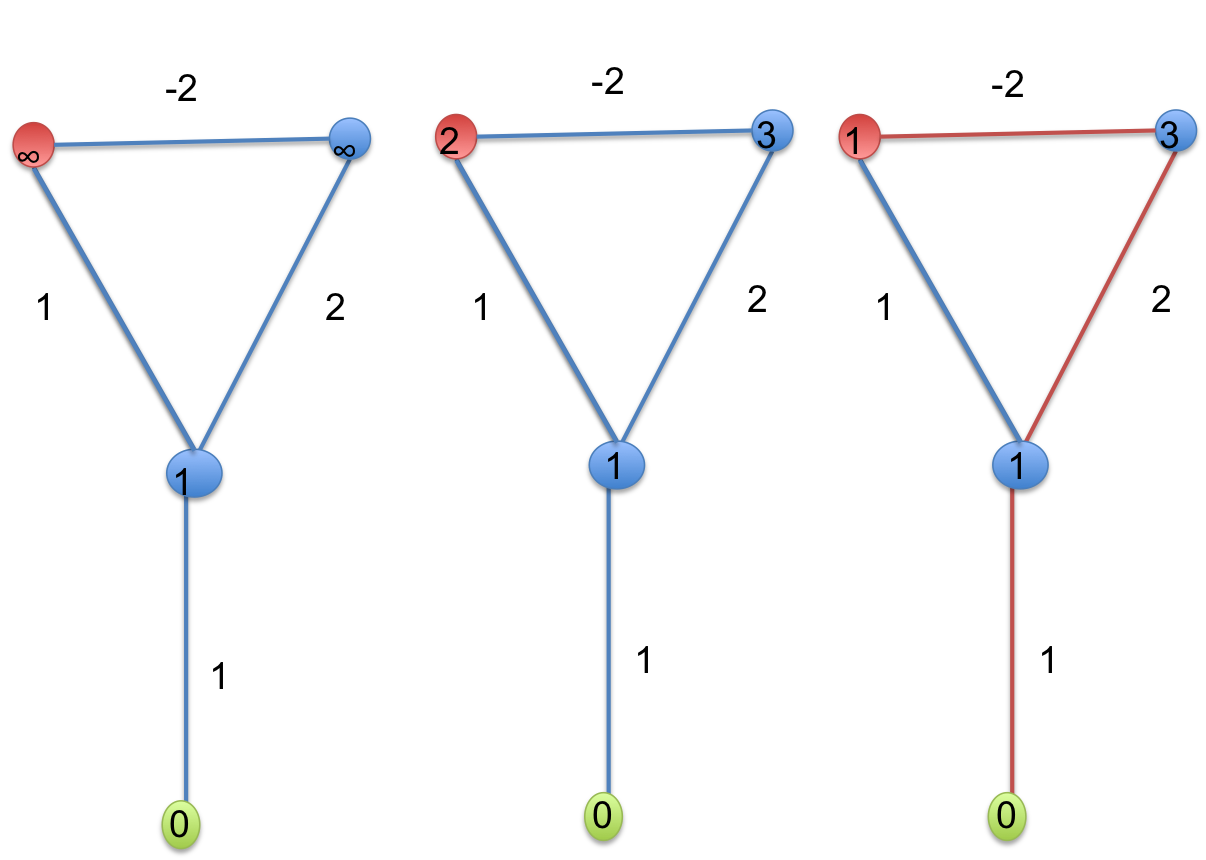
\includegraphics[width=0.60\textwidth]{images/fig1}
		\end{center}
		Because there are $4$ vertices, every edge will be relaxed $3$
		times. We can report the shortest path from green to red (or
		from green to any node) after the algorithm has run by repeatedly taking the predecessor of
		our end node.
		\item 
			Let $V = \{v_1,v_2,...v_n\}$ and $E =
			\{(v_1,v_2),(v_2,v_3),...,(v_{n-1},v_n)\}$
			if $s= v_1$ and $v= v_n$. After $\Omega(n^2)$ operations
			$d[v] = \infty$ but it will be correct by the time the
			algorithm terminates.
		\item
		\begin{enumerate}
			\item  For this algorithm to run in $\Omega(n^2)$
				time, for every node I would only store $d[v_i]$, its list
				of edges, and whether or not it has been
				expanded. I would NOT use a priority queue
				to slow down the algorithm from
				$\Omega(m+n\log n)$ to $\Omega(n^2)$. Instead  I
				would simply store the fringe as a list, and every time
				search it in linear time for the lowest $d$
				value on the fringe. Because there are a maximum of $n$ nodes
				on the fringe and in the worst case scenario I
				would have to pick every node out of the fringe
				to expand it, the runtime here would be on the
				order of $\Omega(n^2)$
			\item I would store the same attributes as above only
				this time I would use a priority queue for the
				fringe to bring Dijkstra's algorithm back down to the
				expected runtime. 
			\item For every node $v_i$, I would store $d[v_i]$, a list
				of its edges and its predecessor (that is the
				last node that overrode its distance value).
				The worst case time is $O(nm)$, so our
				runtime goals are satisfied by the original
				algorithm. \footnote{That is: for $i$ in range
				$1,n-1$ check every edge $e_{r,s}$ of weight $w$ from nodes
				$v_r$ to $v_s$ and if $d[v_r] + w < d[v_s] $ set
				$d[v_s] = d[v_r] + w$, and set $v_r$ to be the
				predecessor of $v_s$. Pretty clearly we can see
				the expected and worst case runtime of this
				algorithm is the number of nodes times the
				number of edges.}
		\end{enumerate}
		\item 
		\textbf{Algorithm}\\
		\textbf{Searching}
		Create an array $d$ to store $|V|$ numbers, one for each vertex.
		Create an array $p$ to store $|V|$ pointers to vertices, one for each vertex.
		This is the array we will use to keep track of the predecessor
		for any given vertex.
		Set $d[s] = 0$ and all other elements of $d$ to $\infty$.
		Let $v_1,v_2,...,v_n$ be all elements with orders between $t$
		and $s$ read in there topological order.
		\begin{alltt}
		For i = 1 to i = n: 
		  For all neighbors 'r' of v_i:
		    if d[v_i] + w < d[r]: (w = edge weight between v_i and r)
				      d[r] = w + d[v_i]
				      p[r] = v_i
		\end{alltt}
		\textbf{Reporting}
		Recursively record the predecessor of $s$ until you get back to
		$t$, reverse this list and report it.\\
		\textbf{Correctness}
		Let $T(v)$ be the topological order for any vertex $v$.
		No vertex can have an edge to a vertex with a lower
		topological order (either directly or by induction indirectly).
		So updating $d[a]$ for a vertex $a$ will not
		change $d[b]$ if $T(a) < T(b)$. This means that $d[s]$ will never change from
		us expanding vertices of lower topological order. When we expand
		the node after $s$ in topological order call it $r$. We know
		$d[r]$ will never change, that is to say we know there can't be
		a path from $s$ to 
		anything after $r$ back $r$ so $d[r]$ must be correct. By
		induction on this idea once 
		we get to $t$, $d[t]$ must be correct and every predecessor must
		be set correctly. \\
		\textbf{Runtime}
		First note that there are $O(|V|)$ elements with topological
		orders between $s$, $t$. Reading elements in order by one off
		the ordering we have to check every edges of every vertices in this
		list.
		If you assume the number of edges per vertex is constant our runtime is 
		$$O(|V|c) = O(|V|)$$
		However notice that we are checking every edge for $O(|V|)$
		vertices so this may be $O(|E|)$ in itself giving us a final
		runtime of if you don't assume a constant number of edges
		$$O(|V|+|E|)$$.
		\item
		\textbf{Algorithm}
		The algorithm here is the same as in the last question the only
		thing we need to change is to set all values of $d$ except for
		$d[s]$ to $-1$ and change the if statement from
		\item
		\textbf{Algorithm}
		Add two vertices to the graph, one with zero weight edges to all
		blue points, and another with zero weight edges from every orange
		point to itself. We will consider these two nodes our start and
		end points. \\
		For every vertex of the graph, eliminate every edge to vertex
		with an $x$ coordinate lower then or equal to its own. This will make the graph
		only flow one way, and there will be no cycles. That is to say it is
		now a DAG. So we can apply a topological sort to order the
		vertices of our DAG.
		For every remaining edge of the graph, set its edge weight to be the
		euclidean distance between the points that the start and end
		vertices represent. Now run the algorithm above for shortest
		path on a DAG described in question 6.
		\textbf{Correctness} 
		Suppose there exists a shorter path between a orange node and a
		blue node then the one we found in this algorithm. This implies
		that there is a shorter path between our start and end vertices,
		as the distance between our start and end vertices is the same
		as the minimum distance between any blue node and any orange
		node.\\
		We can also see intuitively that removing the edges that
		decrease our $x$ coordinate does not impact the shortest path
		through the graph, as no shortest path would ever include steps
		that traveled in the negative $x$ direction.
		In addition, because our edge weights correspond to euclidean
		distance, we know that this is the minimum distance path by
		correctness of the shortest path of a DAG.\\
		\textbf{Runtime}
		The runtime to remove every backwards edge and compute the
		distance between any two points with an edge are both on the
		order $O(|E|)$. A topological sort runs in $O(|E| + |V|)$ time
		and the shortest path algorithm for a sorted DAG also runs in
		$O(|E| + |V|)$ time.
		\item I would use divide an concer to break up the shortest path
			problem into sub-problems at different scales then takel
			those sub problems with Dijkstra algorithm.
			to start divide the map of the USA into one square mile
			"blocks." For each of these blocks I would create graphs
			with edges representing the roads and vertices
			representing houses in that block. Finding the shortest
			path within a block could be done with Dijkstra's algorithm,
			as the number of edges and vertices within one block
			should be much more manageable then the whole map.
			For every block I would also compute the shortest path
			between each of its corners, e.g. the shortest path
			from the south west corner to the north west corner.
			To answer shortest path questions between blocks, I would
			create a graph where the north west corner of each block
			was a vertex with 
			edges to other blocks that corresponded to the distance
			to travel to any adjacent block.
			First we could use Dijkstra's algorithm on the blocks
			graph to find the shortest path between any one of the
			four corners, the block you start in to any one of the
			four corners of the block you finish in. Then we could
			use Dijkstra's algorithm to get  from your start
			to the corner of the block your path starts from and
			from the place your path stops to your destination.
			Below is an illustration of the algorithm 
			\begin{center}
				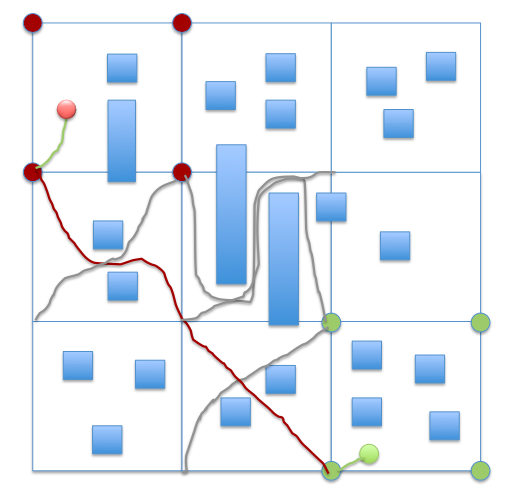
\includegraphics[width=0.6\textwidth]{images/fig2}
			\end{center}
			Gray paths are the pre-computed paths between blocks (drawn in
			only 3 squares), red paths are the paths the algorithm
			has chosen between blocks, and green paths are the paths
			between endpoints and the main path.
			Note that this algorithm does not necessarily find the
			minimum path, as any path between blocks must pass
			through some corner of a block but in a problem like
			finding the shortest path from the east coast to the west
			coast this distance should be relatively small. If the
			search space on the block graph is still too large you
			could combine $10$ by $10$ chunks of blocks in the same
			way that we constructed a graph of blocks (calculating the
			shortest path between chunks from the shortest paths
			across individual blocks) and do a
			Dijkstra search on that graph before we go down to the
			level of blocks. We see how we can add higher level
			graphs to get good ideas of how to get from one general
			area to another, and lower level graphs to get from the
			startpoint or to the endpoint from any given area.
			\item 
			If there is a negative weight cycle there would be a
			negative entry along the main diagonal of your output.
			To see why this first note that any negative weight
			cycle must trivially contain $|V|$ or fewer nodes.
			Let $a_1 \rightarrow a_2 \rightarrow ... \rightarrow a_n
			\rightarrow a_1$
			then the shortest path between $a_1$ and itself 
			with $|V|$ or fewer nodes is one or more loops through the 
			negative cycle. Because the algorithm always 
			finds the shortest path (with $|V|$ or fewer nodes) it
			will find this one so the distance of the shortest path from $a_1$ to
			itself will negative in the output.
		\item The output matrix from the Warshall-Floud algorithm gives us
			$\delta(a,b)$ (that is the \textit{length of} the
			shortest path for $a$ to $b$. For any two vertices of our graph $a,b$ to
			find a shortest path from $a$ to $b$ note that if a node
			$c$ is along this path
			$$\delta(a,b) = \delta(a,c) + \delta(c,b)$$
			And we know that at least one neighbor of $a$ must be
			along a shortest path so check every neighbor of $a$ to see if
			they meet this criterion. Once we've found one that does
			we can report $a$, consider the node we found our
			startpoint and repeat the algorithm above until we
			arrive at
			$b$.\\
			To prove that this algorithm runs in optimal time note
			that we are reporting $k$ elements where $k$ is the
			number of vertices along the shortest path. Because $k$ is
			on the order of $|V|$ we know that the number of
			operations it takes to
			report our solution alone means this algorithm must run
			in $O(|V|)$ time. So a solution is optional if it
			runs in linear time.
			Because every node has an assumed constant number of
			neighbors we only need to check a fixed number of edges
			per node till we find the next that vertex that
			satisfies the
			equation above, this will be the next vertex along the shortest
			path. Meaning our solution runs in constant time per
			vertex, and linear time altogether. Hence our
			solution is optimal.
\end{enumerate}
\end{document}

